\chapter{Konzeption des Modells}
\label{chap:konzept}
\section{Datensatz}
Analog zu der in Kapitel \ref{chap:vorherige-arbeiten-rub} beschriebenen Arbeit wird der \ac{GTSRB} als Datensatz für diese Studienarbeit verwendet. Dies hängt mit der Größe des Datensatzes zusammen, mit der vergleichsweise kleinen Auflösung der einzelnen Bilder und damit, dass sich diese Arbeit auf die Genereriung deutscher Straßenschilder beschränkt. Es soll jedoch in Kapitel \ref{chap:Evaluation} ebenfalls geprüft werden, inwiefern das Resultat der Arbeit genutzt werden kann, um Bilder zu generieren, die Straßenschilder aus anderen Ländern zeigen. Länder, die das Wiener Übereinkommen über Straßenschilder unterzeichnet haben, besitzen vergleichsweise ähnlich aussehende Straßenschilder. Durch das Übereinkommen wird mitunter die grundlegende Form und Farbe verschiedener Schilder bestimmt. \cite{GTSRB} \cite{vienna-convention}

Der \ac{GTSRB} besteht aus mehr als 50.000 Bildern verteilt auf 43 Klassen respektive 43 verschiedenen Arten von Straßenschildern. Beispiele aus dem Datensatz sind in folgender Abbildung dargestellt. \cite{GTSRB}
\begin{figure}[H]
   \centering
   \begin{subfigure}[b]{0.125\textwidth}
       \centering
       \includegraphics[height=\textwidth]{../images/GTSRB/00093.png}
       \caption{}
       \label{fig:gtrsb-paper-bsp-image-1}
   \end{subfigure}
   \hspace{3em}%
   \begin{subfigure}[b]{0.125\textwidth}
       \centering
       \includegraphics[height=\textwidth]{../images/GTSRB/00847.png}
       \caption{}
       \label{fig:gtrsb-paper-bsp-image-2}
   \end{subfigure}
   \hspace{3em}%
   \begin{subfigure}[b]{0.125\textwidth}
       \centering
       \includegraphics[height=\textwidth]{../images/GTSRB/00040.png}
       \caption{}
       \label{fig:gtrsb-paper-bsp-image-3}
   \end{subfigure}
   \hspace{3em}%
   \begin{subfigure}[b]{0.125\textwidth}
    \centering
    \includegraphics[height=\textwidth]{../images/GTSRB/00052.png}
    \caption{}
    \label{fig:gtrsb-paper-bsp-image-4}
\end{subfigure}
      \caption{Beispielbilder aus dem \acs{GTSRB} Datensatz \cite{GTSRB}}
      \label{fig:gtrsb-paper-bsp-images}
\end{figure}

Die Bilder des Datensatzes besitzen unterschiedliche Seitenverhältnisse und verschiedene Auflösungen. Ein Großteil der Bilder ist jedoch kleiner als 100x100 Pixel. Die Bilder basieren auf Videos, die durch die Autoren tagsüber im Straßenverkehr aufgenommen wurden. Die Trainingsbilder sind ungleich auf die Anzahl an Klassen verteilt. Dies hängt mitunter damit zusammen, dass die jeweiligen Schilder nicht gleich häufig im Straßenverkehr verwendet werden. Unterteilt wird der Datensatz in 39.209 Trainingsbilder und 12.630 Testbilder. Da das Ziel dieser Arbeit jedoch nicht ist, einen Klassifikator mit den generierten Bildern zu trainieren, können auch die Testbilder für das Training des Netzes verwendet werden. Es wird nicht zwischen Trainings- und Testbildern unterschieden. \cite{GTSRB}

Der Datensatz wird in dieser Arbeit zunächst so präpariert, dass nur Bilder für das Training verwendet werden, die mindestens 50 Pixel breit oder hoch sind. Dies wird im Verlauf geändert, sodass die Mindestgröße 75 Pixel beträgt.

Die Verteilung der Daten ist auch im präparierten Datensatz nicht homogen. Die nachfolgenden Diagramme zeigen die Verteilung der Daten innerhalb des präparierten Datensatzes. Für die Erhebung mussten die Testdaten manuell ihren Klassen zugeordnet werden.

\definecolor{plotcolor}{HTML}{2b2b2b}

\begin{figure}
\centering
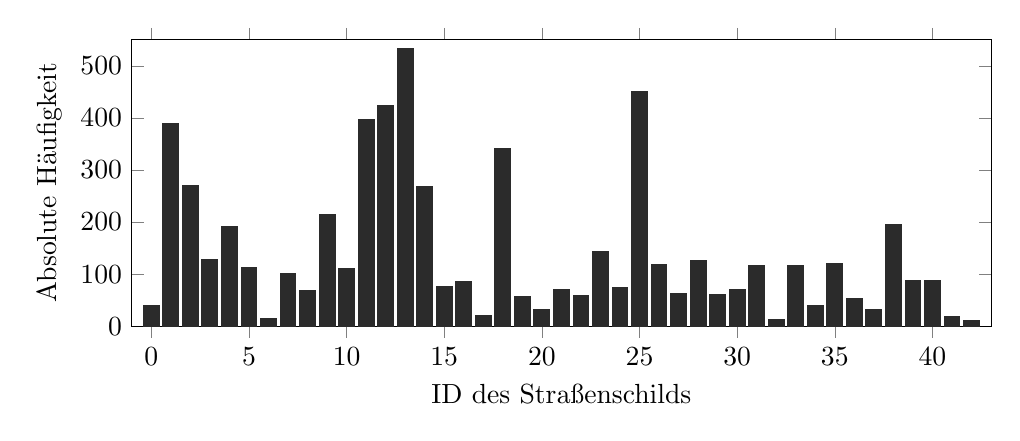
\begin{tikzpicture}
    \begin{axis} [ybar, ylabel={Absolute Häufigkeit}, xlabel={ID des Straßenschilds}, width=\linewidth*0.9, height=\linewidth*0.3, scale only axis=true, xmin=-1, xmax=43, ymin=0, ymax=550, bar width=0.2cm, ytick={0, 100, 200, 300, 400, 500}]
    \addplot[plotcolor, fill] coordinates {
        (0, 40)
        (1, 390) 
        (2, 270) 
        (3, 127)
        (4, 192)
        (5, 113)
        (7, 101)
        (8, 69)
        (11, 396)
        (18, 342)
        (19, 56)
        (20, 31)
        (21, 70)
        (22, 58)
        (23, 144)
        (24, 75)
        (25, 451)
        (26, 118)
        (27, 62)
        (28, 126)
        (29, 60)
        (30, 71)
        (31, 117)
        (6, 14)
        (9, 214)
        (10, 110)
        (12, 424)
        (13, 534)
        (14, 269)
        (15, 77)
        (16, 85)
        (17, 21)
        (32, 12)
        (33, 116)
        (34, 39)
        (35, 121)
        (36, 53)
        (37, 31)
        (38, 195)
        (39, 87)
        (40, 88)
        (41, 19)
        (42, 10)
    };
    \end{axis}
\end{tikzpicture}
\caption{Häufigkeitsverteilung der Arten von Straßenschildern im präparierten Datensatz}
\end{figure}

\begin{figure}
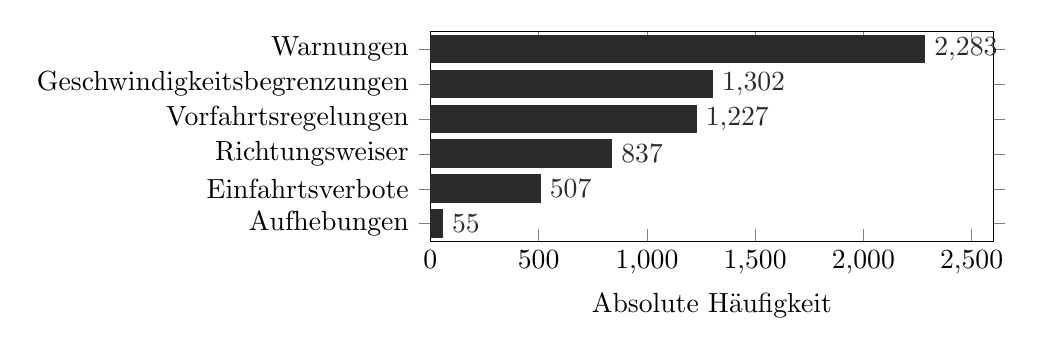
\begin{tikzpicture}
\begin{axis}[ 
xbar, xmin=0, height=\linewidth*0.35, width=\linewidth*0.72,
xlabel={Absolute Häufigkeit},
symbolic y coords={
    Aufhebungen, 
    Einfahrtsverbote,
    Richtungsweiser,
    Vorfahrtsregelungen,
    Geschwindigkeitsbegrenzungen,
    Warnungen,
    },
ytick=data,
nodes near coords, 
nodes near coords align={horizontal},
ytick=data, xmax=2600, xtick={0, 500, 1000, 1500, 2000, 2500}
]
\addplot[plotcolor, fill] coordinates {
    (1227,Vorfahrtsregelungen)
    (1302,Geschwindigkeitsbegrenzungen) 
    (837,Richtungsweiser)
    (55,Aufhebungen)
    (507,Einfahrtsverbote) 
    (2283,Warnungen)};
\end{axis}
\end{tikzpicture} %width=6cm,height=7.59cm
\caption{Häufigkeitsverteilung der Kategorien von Straßenschildern im präparierten Datensatz}
\end{figure}

\section{Framework}
\paragraph{Tensorflow Addons}
\paragraph{Tensorflow Graphics}
Erklären: Wieso benutze ich, wo möglich, Tensorflow Graphics statt OpenCV? Wieso gibt es Tensorflow Graphics überhaupt?
\paragraph{OpenCV}
Erwähnen: OpenCV wird nur da benutzt, wo keine Tensorflow funktionen verwendet werden können. Beeinträchtigt die Performance.

\section{Architektur}
In Kapitel \ref{chap:NoGANs} werden verschiedene generative Netzwerkarchitekturen vorgestellt. Zunächst soll darauf eingegangen werden, welche dieser Herangehensweisen gewählt wird. Jede der Architekturen besitzt ihre Vor- und Nachteile. Der größte Nachteil von \acp{PixelRNN} ist, dass die Pixel eines Bildes nicht parallel zueinander generiert werden können. Dies verlangsamt die Generierung und damit das Training des Modells.

\textbf{Entscheidungsmatrix?}

\section{Datenaugmentation}
Bevor die Piktogramme an den Generator übergeben werden, werden sie zufällig rotiert. Dadurch muss der Generator die Rotation nicht eigenständig lernen und dieser Aspekt der Generierung lässt sich deterministisch bestimmen. Dabei soll die Rotation nicht nur in x-y-Richtung erfolgen, sondern auch eine dreidimensionale Rotation simuliert werden. Und zwar so, als sei das Schild aus einer beliebigen Frontalperspektive aufgenommen worden.

Um bestimmte Transformationen eines Bilds mittels einer Matrixpultiplikation darstellen zu können, wird häufig ein sogenanntes \emph{homogenes Koordinatensystem} verwendet. Dabei wird das Koordinatensystem um eine weitere Dimension erweitert. Ein Punkt $p = [x, y]^\mathsf{T}$ kann somit um einen beliebigen Wert in z-Richtung verschoben werden. Dadurch wird ein Punkt $\tilde{p}$ im homogenen Koordinatensystem durch drei Koordinaten $\tilde{x}$, $\tilde{y}$ und $\tilde{z}$ beschrieben. Transormationen werden in der homogenen Darstellung durchgeführt und anschließend werden daraus die kartesischen Koordinaten $x$ und $y$ bestimmt. Somit erhält man aus der Transformation erneut ein zweidimensionales Bild. \cite{geometric-ops} \cite{math-primer}

Dies wird für eine dreidimensionale Rotation der Piktogramme benötigt. Die Rotation soll durch drei \emph{eulersche Winkel} beschrieben werden. Das bedeutet, dass sie sich aus einer Rotation um die z-Achse, einer um die y-Achse und einer um die x-Achse zusammensetzt. Dies ist in der nachfolgenden Grafik abgebildet. Die bläulichen Balken zeigen dabei die Achse an, um die gedreht wird. Die erste Rotation ist um die z-Achse, wodurch der Balken in die dritte Bildebene geht. \cite{math-primer}

\begin{figure}[H]
	\centering
	\includegraphics[width=0.8\textwidth]{../images/3 Konzeption des Generative Adversarial Networks/Datenaugmentation/Rotation.png}
	\caption{Rotation der Straßenschilder mittels eulerscher Winkel}
	\label{fig:rotation}
\end{figure}

%\begin{figure}[H]
%    \centering
%    \begin{subfigure}[b]{0.2\textwidth}
%        \centering
%        \includegraphics[height=\textwidth]{../images/3 Konzeption des Generative Adversarial Networks/Datenaugmentation/z-axis.png}
%        \caption{Rotation um die z-Achse (\emph{rollen})}
%    \end{subfigure}
%    \hspace{3em}%
%    \begin{subfigure}[b]{0.2\textwidth}
%        \centering
%        \includegraphics[height=\textwidth]{../images/3 Konzeption des Generative Adversarial Networks/Datenaugmentation/y-axis.png}
%        \caption{Rotation um die y-Achse \emph{}}
%    \end{subfigure}
%    \hspace{3em}%
%    \begin{subfigure}[b]{0.2\textwidth}
%        \centering
%        \includegraphics[height=\textwidth]{../images/3 Konzeption des Generative Adversarial Networks/Datenaugmentation/x-axis.png}
%        \caption{Rotation um die x-Achse}
%    \end{subfigure}
%    \caption{Rotationen mittels eulerscher Winkel}
% \end{figure}

Jede Rotation ist durch einen einzelnen Winkel um die jeweilige Achse bestimmt. Kombiniert man die Rotationen, kann die resultierende Tranformation somit durch drei Winkel $(\alpha_z, \alpha_y, \alpha_x)$ eindeutig beschrieben werden. Für die Erzeugung einer zufälligen Rotation müssen randomisierte Werte für diese Winkel bestimmt werden. \cite{math-primer}

Zusätzlich zu der Rotation, soll das Modell die Piktogramme zufällig in ihrer Größe skalieren. Die genannten Augmentationen dienen dazu, die Verteilung der real aufgenommenen Schilder abbilden zu können. Im Datensatz besitzen die Schilder eine unterschiedliche Größe und sind aus verschiedenen Perspektiven aufgenommen. Dadurch dass die Augmentation deterministisch ist, kann sie dazu genutzt werden, um gezielt nur Bilder durch das Modell zu generieren, die aus bestimmten Perspektiven und mit festgelegten Größen generiert wurden. Alternativ kann auch die randomisierte Augmentation beibehalten werden, um eine möglichst große Bandbreite an unterschiedlichen Bildern zu erzeugen.

%Eine Rotation in x- und y-Richtung besitzt folgende sogenannte \emph{Transformationsmatrix} \cite{geometric-ops}:

%\begin{equation}
%    \begin{bmatrix}
%        \cos{\theta} & -\sin{\theta} & 0\\
%        \sin{\theta} & \cos{\theta} & 0\\
%        0 & 0 & 1
%    \end{bmatrix}
%\end{equation}

%Um ein Bild zu Rotieren, multipliziert man in der homogenen Darstellung jeden Pixel des Bilds mit dieser Matrix. Die Winkel $\theta$ sollten alle gleich groß sein, damit das Bild durch die Rotation nicht verzerrt wird. Für die Rotation der Piktogramme der Straßenschilder wird diese Matrix um eine Rotation in z-Richtung erweitert. Die vollständige Gleichung sieht damit wie folgt aus:

%\begin{equation}
%    \begin{bmatrix} \tilde{x} \\ \tilde{y} \\ \tilde{z} \end{bmatrix}
%    =
%    \begin{bmatrix}
%        \cos{\theta_{xy}} & -\sin{\theta_{xy}} & 0\\
%        \sin{\theta_{xy}} & \cos{\theta_{xy}} & 0\\
%        0                 & \sin{\theta_{z}} & 1
%    \end{bmatrix}
%    \cdot \begin{bmatrix} x \\ y \\ 1 \end{bmatrix}
%\end{equation}

%Die linke Seite der Gleichung zeigt $\tilde{p}$, das Ergebnis der Rotation im dreidimensionalen Raum. Die Rotationsmatrix wird dafür mit der homogenen Darstellung des zweidimensionalen Punktes $p$ multipliziert. Die letzte Zeile der Rotationsmatrix stellt die Rotation in z-Richtung dar. Der Term $\sin{\theta_{z}}$ verändert die Pixelwerte in y-Richtung, das heißt das Piktogramm wird in z-Richtung geneigt. Rückblickend wäre jedoch auch eine Rotation in x-Richtung sinnvoll. Dadurch würde der Effekt entstehen, das Foto sei von der Seite aufgenommen worden. Die Rotation der Piktogramme in z-Richtung soll weitaus subtiler sein als in x- und y-Richtung. Deshalb ist $\theta_{z}$ allgemein kleiner als $\theta_{xy}$. \cite{geometric-ops}

%Für die programmatische Implementierung der Rotation mit dem Framework OpenCV muss die Überführung des Bildes aus der homogenen Darstellung zurück in den zweidimensionalen Raum nicht manuell erfolgen. Deshalb soll darauf nicht weiter eingegangen werden. Grundsätzlich wäre dies jedoch der nächste Schritt, um das rotierte Schild in einem zweidimensionalen Bild darstellen zu können.

%\begin{listing}[H]
%    \caption{Rotation der Piktogramme mit OpenCV}
%    \begin{minted}[fontsize=\footnotesize, linenos, breaklines, autogobble]{python}
%        def apply_3d_rotation(img_tensor, theta_xy, theta_z, image_size):
%            """
%            Rotate the img_tensor in x, y and z direction.
%            """
%            transformation_matrix = np.array([
%                [np.cos(theta_xy), -np.sin(theta_xy), 0],
%                [np.sin(theta_xy),  np.cos(theta_xy), 0],
%                [0,                 np.sin(theta_z),  1] 
%            ])
%            rotated_image = cv2.warpPerspective(img_tensor.numpy(), transformation_matrix, (image_size, image_size))
%            return rotated_image
%    \end{minted}
%\end{listing}

%\begin{lstlisting}[language=Python, caption={Rotation der Piktograme mit OpenCV}]
%def apply_3d_rotation(img_tensor, theta_xy, theta_z, image_size):
%    """
%    Rotate the img_tensor in x, y and z direction.
%    """
%    transformation_matrix = np.array([
%    [np.cos(theta_xy), -np.sin(theta_xy), 0],
%    [np.sin(theta_xy),  np.cos(theta_xy), 0],
%    [0,                 np.sin(theta_z),  1] 
%    ])
%    rotated_image = cv2.warpPerspective(img_tensor.numpy(), transformation_matrix, (image_size, image_size))
%    return rotated_image    
%\end{lstlisting}

\section{Training}
Überlicherweise soll beim Training von neuronalen Netzen die Verlustfunktion gegen den Wert \emph{null} streben. Bei diesem Modell soll die Verlustfunktion jedoch gegen einen Wert konvergieren, der größer ist als \emph{null}. In diesem Fall schaffen es weder die Generatoren, die Funktionswerte zu minimieren, noch können die Diskriminatoren die Funktionswerte weiter maximieren. In diesem Fall ist das sogenannte \emph{Nash-Gleichgewicht} erreicht. Das Training ist somit beendet, da sich das Modell mit den gegebenen Daten nicht weiter verbessern kann.